\documentclass{beamer}
\usetheme[
  block=fill,
  background=dark,
  titleformat=smallcaps,
  progressbar=frametitle,
  numbering=none,
]{metropolis}

% st
\usepackage{ulem}

% smileys
\usepackage{wasysym}

% cross-reference other files
\usepackage{xr}

% url
\usepackage{hyperref}

% math
\usepackage{amsmath}
\usepackage{amssymb}
\usepackage{mathtools}
\usepackage{proof}
\usepackage{stmaryrd}
% theorem
\newtheorem{defn}{Definition}[section]
% Decorated Arrow
\newlength{\arrow}
\settowidth{\arrow}{\scriptsize$10$}
\newcommand*{\myrightarrow}[1]{\xrightarrow{\mathmakebox[\arrow]{\text{\scriptsize #1}}}}
% box
\setlength{\fboxsep}{2pt}

\usepackage{rotating}

% color
\usepackage{color}

% graphics
\usepackage{graphicx}
\usepackage{float}
\usepackage{subcaption}

% tikz
\usepackage{tikz}
\usepackage{pgf}
\usetikzlibrary{shapes,external}
\usetikzlibrary{shapes.multipart}
\usetikzlibrary{decorations.pathreplacing}
\usetikzlibrary{matrix}
\usetikzlibrary{calc}

% gloss
\usepackage{linguex} 

% epi
\usepackage{epigraph}

% tabular
\usepackage{tabularx}
\usepackage{booktabs}
\newcolumntype{m}{>{\hsize=.65\hsize}X}
\newcolumntype{s}{>{\hsize=.4\hsize}c}
\newcolumntype{u}{>{\hsize=.25\hsize}X}
\newcolumntype{U}{>{\hsize=.15\hsize}X}
\usepackage{multicol}
\usepackage{multirow}

% algorithm
\usepackage{algpseudocode}
\usepackage{algorithm}

% spacing
\usepackage{setspace}

\title{Extracting \& Learning a Dependency-Enhanced Grammar for Dutch}
\author{Konstantinos Kogkalidis}
\date{June 2019}

\begin{document}
\maketitle

\begin{frame}{Overview}
	\begin{itemize}
	\item Parsing as Deduction
	\item Extraction
	\item Supertagging
	\item Parsing
	\end{itemize}
\end{frame}

\section{Parsing as Deduction}

\begin{frame}{Intro: Categorial Grammars}
\begin{itemize}
	\item Lexicon $\mathcal{L}$: words $\to$ categories
	\item Categories defined by some inductive scheme
	\begin{itemize}
		\item[-] Atomic Categories: full phrases \{\textsc{np}, \textsc{s}, \dots\}
		\item[-] Complex Categories: fractionals \{$\textsc{np}\backslash \textsc{s}$, $\textsc{np}\backslash (\textsc{s}/\textsc{np})$, \dots\}
	\end{itemize}
	\item Category Interactions: Combination Rules
	\item Parsing: Rule Application
\end{itemize}
\end{frame}

\begin{frame}{Intro: Typelogical Grammars}
\begin{itemize}
	\item Lexicon $\mathcal{L}$: words $\to$ \alert{types}
	\item Types defined by some inductive scheme
	\begin{itemize}
		\item[-] Atomic Types: full phrases \{\textsc{np}, \textsc{s}, \dots\}
		\item[-] Complex Types: fractionals \{$\textsc{np}\backslash \textsc{s}$, $\textsc{np}\backslash (\textsc{s}/\textsc{np})$, \dots\}
	\end{itemize}
	\item Type Interactions: \alert{Logical Rules}
	\item Parsing: \alert{Proof Search}
\end{itemize}
\end{frame}

\begin{frame}{Typelogical Grammars: Example (Lambek \& co)}
	\begin{minipage}{0.35\textwidth}
		\small
		\begin{align*}
		\mathcal{L} := 	\text{ducks} &: \textsc{np},  \\
						\text{fish} &: \textsc{np},  \\
						\text{fly} &: \textsc{np}\backslash \textsc{s}, \\
						\text{eat} &: \textsc{np}\backslash (\textsc{s} / \textsc{np}), \\
						\text{majestically} &: (\textsc{np}\backslash \textsc{s}) \backslash (\textsc{np} \backslash \textsc{s})
		\end{align*}
	\end{minipage}\begin{minipage}{0.45\textwidth}
	\scriptsize
		\begin{minipage}{0.6\textwidth}
		    \begin{align*}
		    	\scriptsize
		        \infer{\Gamma, \Delta \vdash B}{
		            \Gamma \vdash B / A
		            &
		            \Delta \vdash A
		        }\tag{/E}\\
		        \\
		        \infer{\Gamma \vdash B/A}{
		            \Gamma, A \vdash B
		        }\tag{/I}
		    \end{align*}
		 \end{minipage}\begin{minipage}{0.6\textwidth}
			    \begin{align*}
			        \infer{\Delta, \Gamma \vdash B}{
			            \Delta \vdash A
			            &
			            \Gamma \vdash A\backslash B
			        }\tag{$\backslash E$}\\
			        \\
			        \infer{\Gamma \vdash A\backslash B}{
			            A, \Gamma \vdash B
			        }\tag{$\backslash I$}
			    \end{align*}		
		\end{minipage}
	\end{minipage}
\end{frame}

\begin{frame}{Directionality \& Lexical Ambiguity}
	\begin{minipage}{0.45\textwidth}
	\begin{align*}
	\mathcal{L} := \text{eten}_1 &: \textsc{np}\backslash (\textsc{s}/\textsc{np}), \\
					\text{eten}_2 &: (\textsc{s}/\textsc{np})/\textsc{np} \\
					\text{eten}_3 &: (\textsc{s}/\textsc{np}), \\
					\text{eten}_{4,5} &: \textsc{np}\backslash (\textsc{np}\backslash \textsc{s}), \\
	\end{align*}
	\end{minipage}\begin{minipage}{0.6\textwidth}
	\small
	\begin{itemize}
		\item[] eenden eten$_1$ vis (SVO)
		\item[] eten$_2$ eenden vis? (VSO)
		\item[] eten$_3$ vis! (VO)
		\item[] eenden die vis eten$_{4,5}$ (SOV / OSV)
	\end{itemize}
	\end{minipage}	
	\centering
		\dots \\
		\vfill
	\pause
		\large
		\frownie
\end{frame}

\begin{frame}{Beyond Directionality: MILL}
	Can we abstract directionality away?\\
	\pause
	Yes: \alert{Multiplicative Intuionistic Linear Logic} (ACG, LP \dots)
	
	\pause
	
	Types:
		\begin{center}{
		$\textsc{T} := \textsc{a} \ | \ \textsc{t}_1 \to \textsc{t}_2 $}
		\end{center}
	
	\pause	
	
	Logical Rules:
	\begin{align*}
    \begin{minipage}{0.5\textwidth}
	\[
        \infer{\Gamma, \Delta \vdash B}{
            \Gamma \vdash A \rightarrow B
            &
            \Delta \vdash A
        }\tag{$\rightarrow$ E}
    \]
    \end{minipage}    \begin{minipage}{0.5\textwidth}
    \[
        \infer{\Gamma \vdash A \rightarrow B}{
            \Gamma, A \vdash B
        }\tag{$\rightarrow I$}\\
    \]
    \end{minipage}
	\end{align*}
\end{frame}

\begin{frame}{MILL - The Good (1): Syntax-Semantics Interface}

	Curry-Howard Correspondence:
	
	\begin{center}{
		MILL $\equiv$ Simply-typed Linear $\lambda$-calculus}
		\pause
		\begin{align*}
		    \begin{minipage}{0.5\textwidth}
				\[
			        \infer{\Gamma, \Delta \vdash f(x): B}{
			            \Gamma: f \vdash A \rightarrow B
			            &
			            \Delta: x \vdash A
			        }
			    \]
			    \end{minipage}    \begin{minipage}{0.5\textwidth}
			    \[
			        \infer{\Gamma \vdash \lambda x. u : A \rightarrow B}{
			            \Gamma, x: A \vdash u: B
			        }
			    \]
	    	\end{minipage}
		\end{align*}
	
	\large
	\smiley	
	\vfill
	\end{center}
\end{frame}

\begin{frame}{MILL: The good (2): Lesser Lexical Ambiguity}
	\begin{align*}
	\mathcal{L} := \text{eten}_1 &: \textsc{np}\backslash (\textsc{s}/\textsc{np}), \\
					\text{eten}_2 &: (\textsc{s}/\textsc{np})/\textsc{np} \\
					\text{eten}_3 &: (\textsc{s}/\textsc{np}), \\
					\text{eten}_{4,5} &: \textsc{np}\backslash (\textsc{np}\backslash \textsc{s}), \\
	\end{align*}
	
	\pause
	\begin{align*}
	\mathcal{L}' := \text{eten}_{1,2,4,5} &: \textsc{np} \to \textsc{np} \to \textsc{s}, \\
					\text{eten}_3 &: \textsc{np} \to \textsc{s}
	\end{align*}

	
	\large
	\center
		\smiley
			\vfill 

\end{frame}


\begin{frame}{MILL - The Bad: Structural Ambiguity}
	\small
	\vfill
	\[
		\infer[\rightarrow E]{\text{eenden}, \text{eten}, \text{vis} \vdash \textsc{s}}{
			\infer[\rightarrow E]{\text{eten}, \text{vis} \vdash \textsc{np} \to \textsc{s}}{
				\infer[\rightarrow Ax.]{\text{eten} \vdash \textsc{np} \to \textsc{np} \to \textsc{s}}{}
				&
				\infer[\rightarrow Ax.]{\text{vis} \to \textsc{np}}{}
				}
			&
			\infer[Ax.]{\text{eenden} \vdash \texttt{eenden}: \textsc{np}}{}			
		}
	\]	
	\center \texttt{(eten vis) eenden}
	\vfill
	\[
	\infer[\rightarrow E]{\text{eenden}, \text{eten}, \text{vis} \vdash \textsc{s}}{
		\infer[\rightarrow E]{\text{eten}, \text{eenden} \vdash \textsc{np} \to \textsc{s}}{
			\infer[\rightarrow Ax.]{\text{eten} \vdash \textsc{np} \to \textsc{np} \to \textsc{s}}{}
			&
			\infer[\rightarrow Ax.]{\text{enden} \to \textsc{np}}{}
			}
		&
		\infer[Ax.]{\text{vis} \vdash \textsc{np}}{}			
	}
	\]
	\texttt{(eten eenden) vis}
	
	\large
	\frownie
	\vfill
\end{frame}

\begin{frame}{Dependency Decorations}
	Replace $\to$ with dependency-decorated variants:
	\begin{itemize}
			\item[] \{$\myrightarrow{su}$, $\myrightarrow{obj}$, $\myrightarrow{predc}$, $\myrightarrow{mod}$, \dots \}
			\item[] eten : $\textsc{np} \myrightarrow{su} \textsc{np} \myrightarrow{obj} \textsc{s}$
	\end{itemize}
	\pause
	Lexical preferences + decorations $\implies$ \alert{reduced ambiguity} \\ 
	\vfill
	\pause
	\alert{Formally}:\\
	Unary modality $\diamondsuit^d$ for $d$ $\in$ \{su, obj, predc, mod, \dots\}\\
    \begin{minipage}{0.4\textwidth}
	\begin{align*}
        \infer{\langle \Gamma \rangle^d \vdash \diamondsuit^d A}{\Gamma \vdash A}\tag{$\diamondsuit^d I$}
	\end{align*}
    \end{minipage}\begin{minipage}{0.6\textwidth}
	\begin{align*}
        \infer{\Gamma [\Delta] \vdash B}{
        \Delta \vdash \diamondsuit^d A
        &
        \Gamma[\langle A \rangle^d] \vdash B
        }\tag{$\diamondsuit^d E$}
	\end{align*}
    \end{minipage}
\end{frame}

\section{Extraction}

\begin{frame}{Extraction: Intro}
	\alert{Goal}\\
	Syntactically-Annotated Corpus $\to$ Type Lexicon
	\vfill
	
	\pause
	\alert{Corpus}\\
	\[
	\text{Lassy-Small:} \quad
		\begin{cases}
			\text{65\,000 Sentences}\\
			\text{1\,000\,000 Words}\\
			\text{$\sim$ 30 Dependency Labels}\\
			\text{$\sim$ 30 POS \& Phrasal Category Tags}\\
		\end{cases}
	\]
\end{frame}

\begin{frame}{Extraction: Parameters}
	\alert{Parameters}
	\begin{itemize}
		\item Translation Tables
			\begin{itemize}
				\item Atomic Types: POS \& Phrasal Category Tags \\
					\{\textit{np}: \textsc{np}, \textit{vnw}: \textsc{vnw}, \dots \}
				\item Implications: Dependency Labels \\
					\{\textit{su}: $\myrightarrow{su}$, \textit{obj}: $\myrightarrow{obj}$, \dots \}
			\end{itemize}
		\item Head Dependencies \\
			\{\textit{hd}, \textit{rhd}, \textit{whd}, \textit{crd}, \textit{cmp}\}
		\item Modifier Dependencies \\
			\{\textit{mod}, \textit{app}, \textit{predm}\}
	\end{itemize}
\end{frame}

\begin{frame}{Extraction: Algorithm}
	\alert{General Idea}
	\begin{itemize}
		\item[] For each branch
			\begin{itemize}
				\item Find head, arguments, modifiers
				\item Collect \& arrange argument types
				\item Type head as a functor from argument types to parent type
				\item Type modifiers as endomorphisms from parent type to itself
			\end{itemize}
	\end{itemize}
	
	\alert{Hypothetical Reasoning}
	\begin{itemize}
		\item[] When type assigning arguments, consider internal ``gaps''
	\end{itemize}
\end{frame}

{
\setbeamercolor{background canvas}{bg=gray!00}
\begin{frame}{Extraction: Example (1)}
	\begin{figure}
		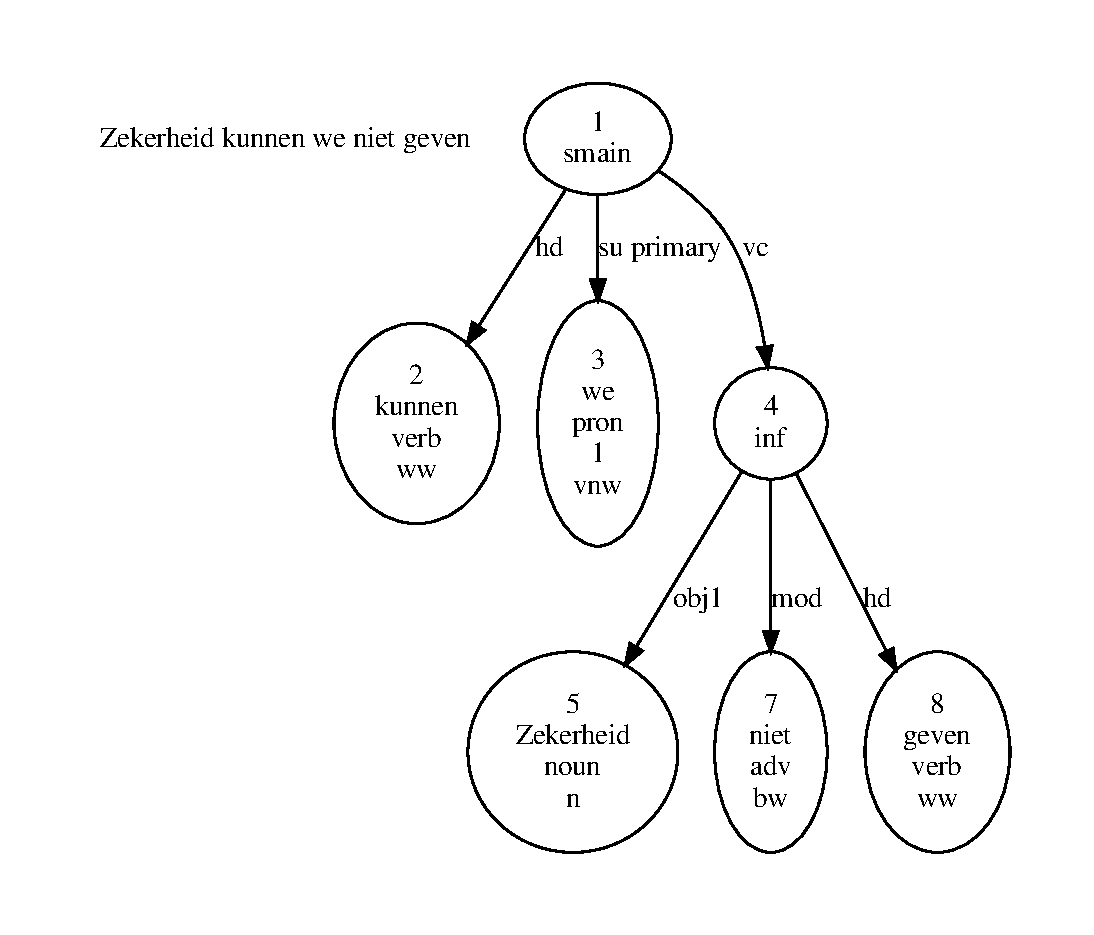
\includegraphics[scale=0.5]{zekerheid.pdf}
	\end{figure}
\end{frame}
}

{
\setbeamercolor{background canvas}{bg=gray!00}
\begin{frame}{Extraction: Example (1)}
	\begin{figure}
		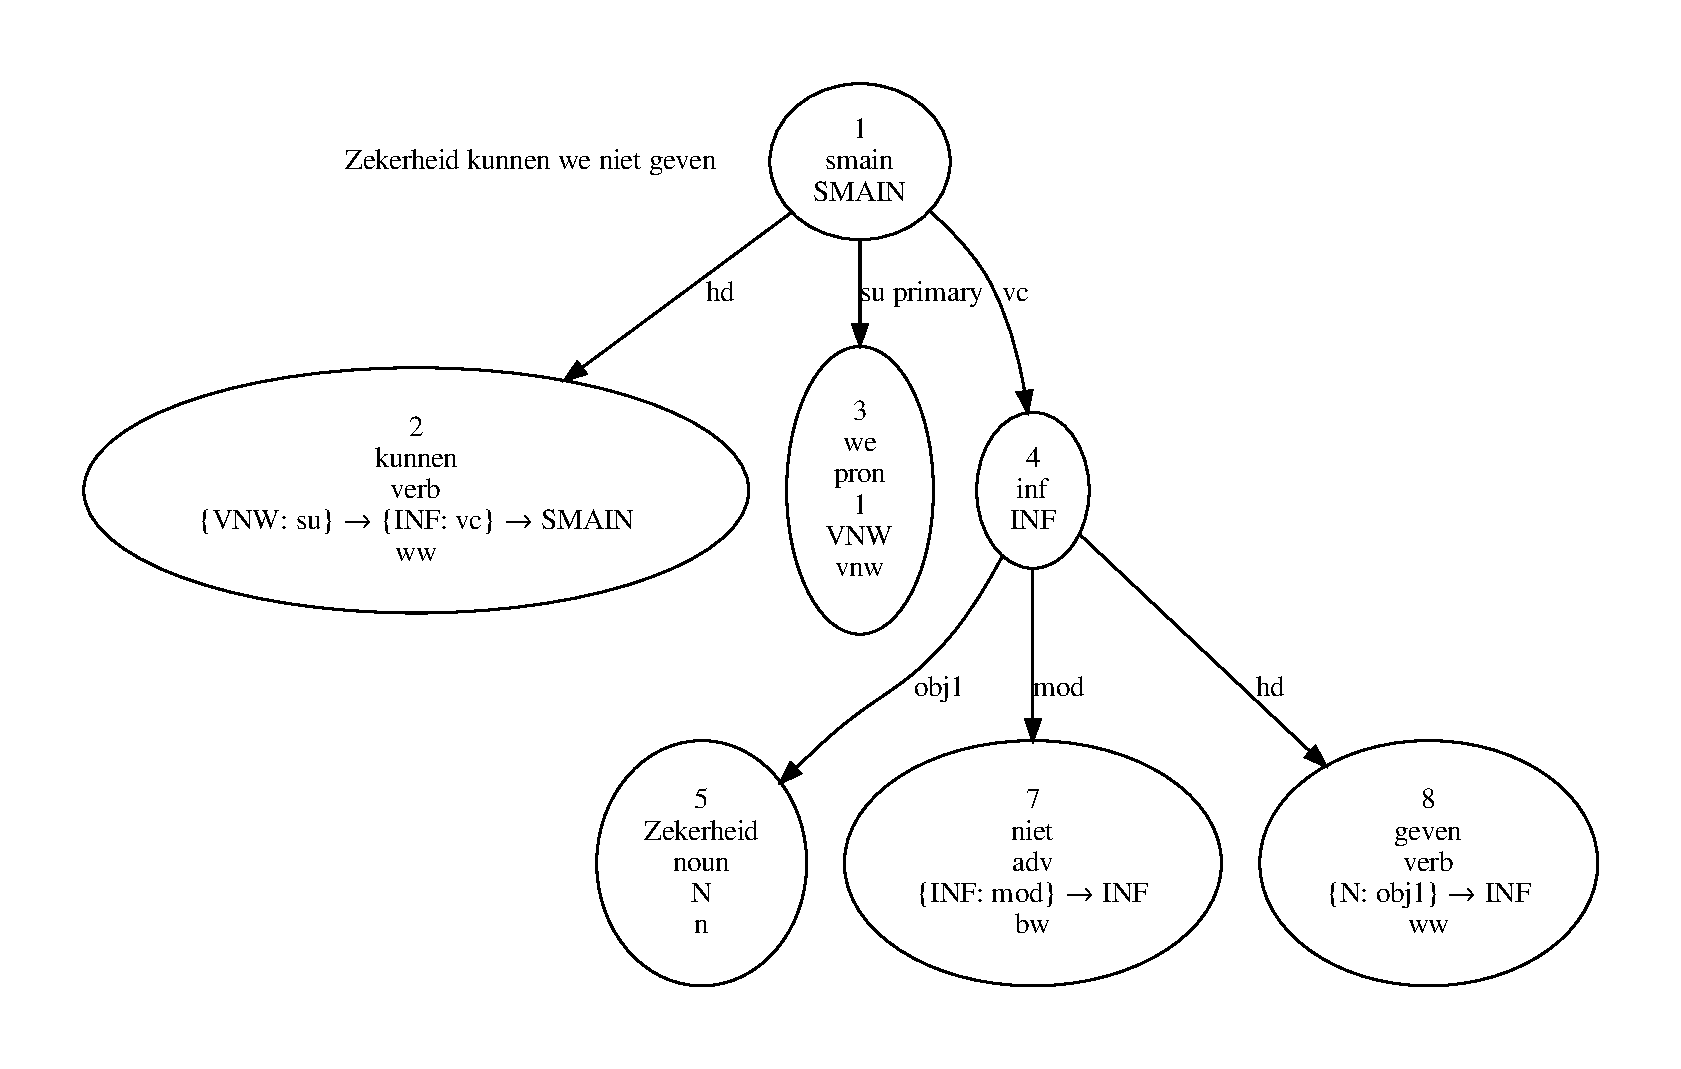
\includegraphics[scale=0.38]{zekerheid2.pdf}
	\end{figure}
\end{frame}
}

{
\setbeamercolor{background canvas}{bg=gray!00}
\begin{frame}{Extraction: Example (2)}
	\begin{figure}
		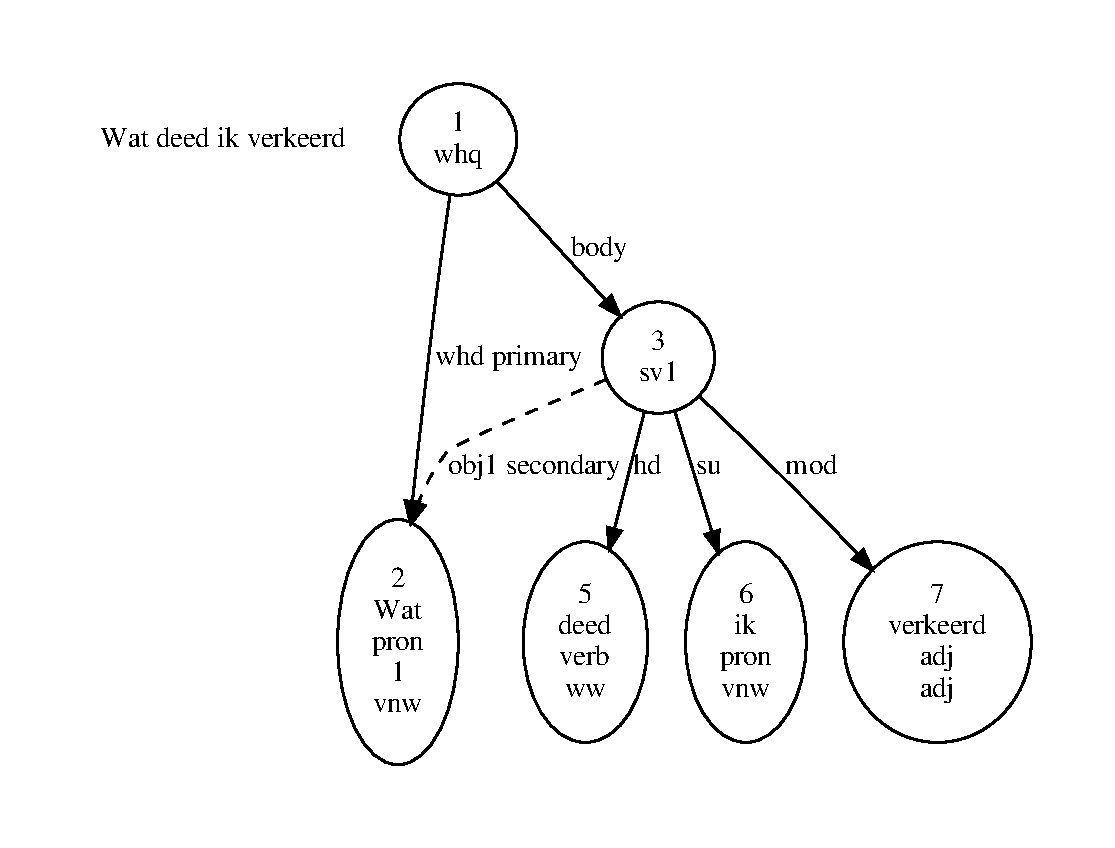
\includegraphics[scale=0.5]{deed.pdf}
	\end{figure}
\end{frame}
}

{
\setbeamercolor{background canvas}{bg=gray!00}
\begin{frame}{Extraction: Example (2)}
	\begin{figure}
		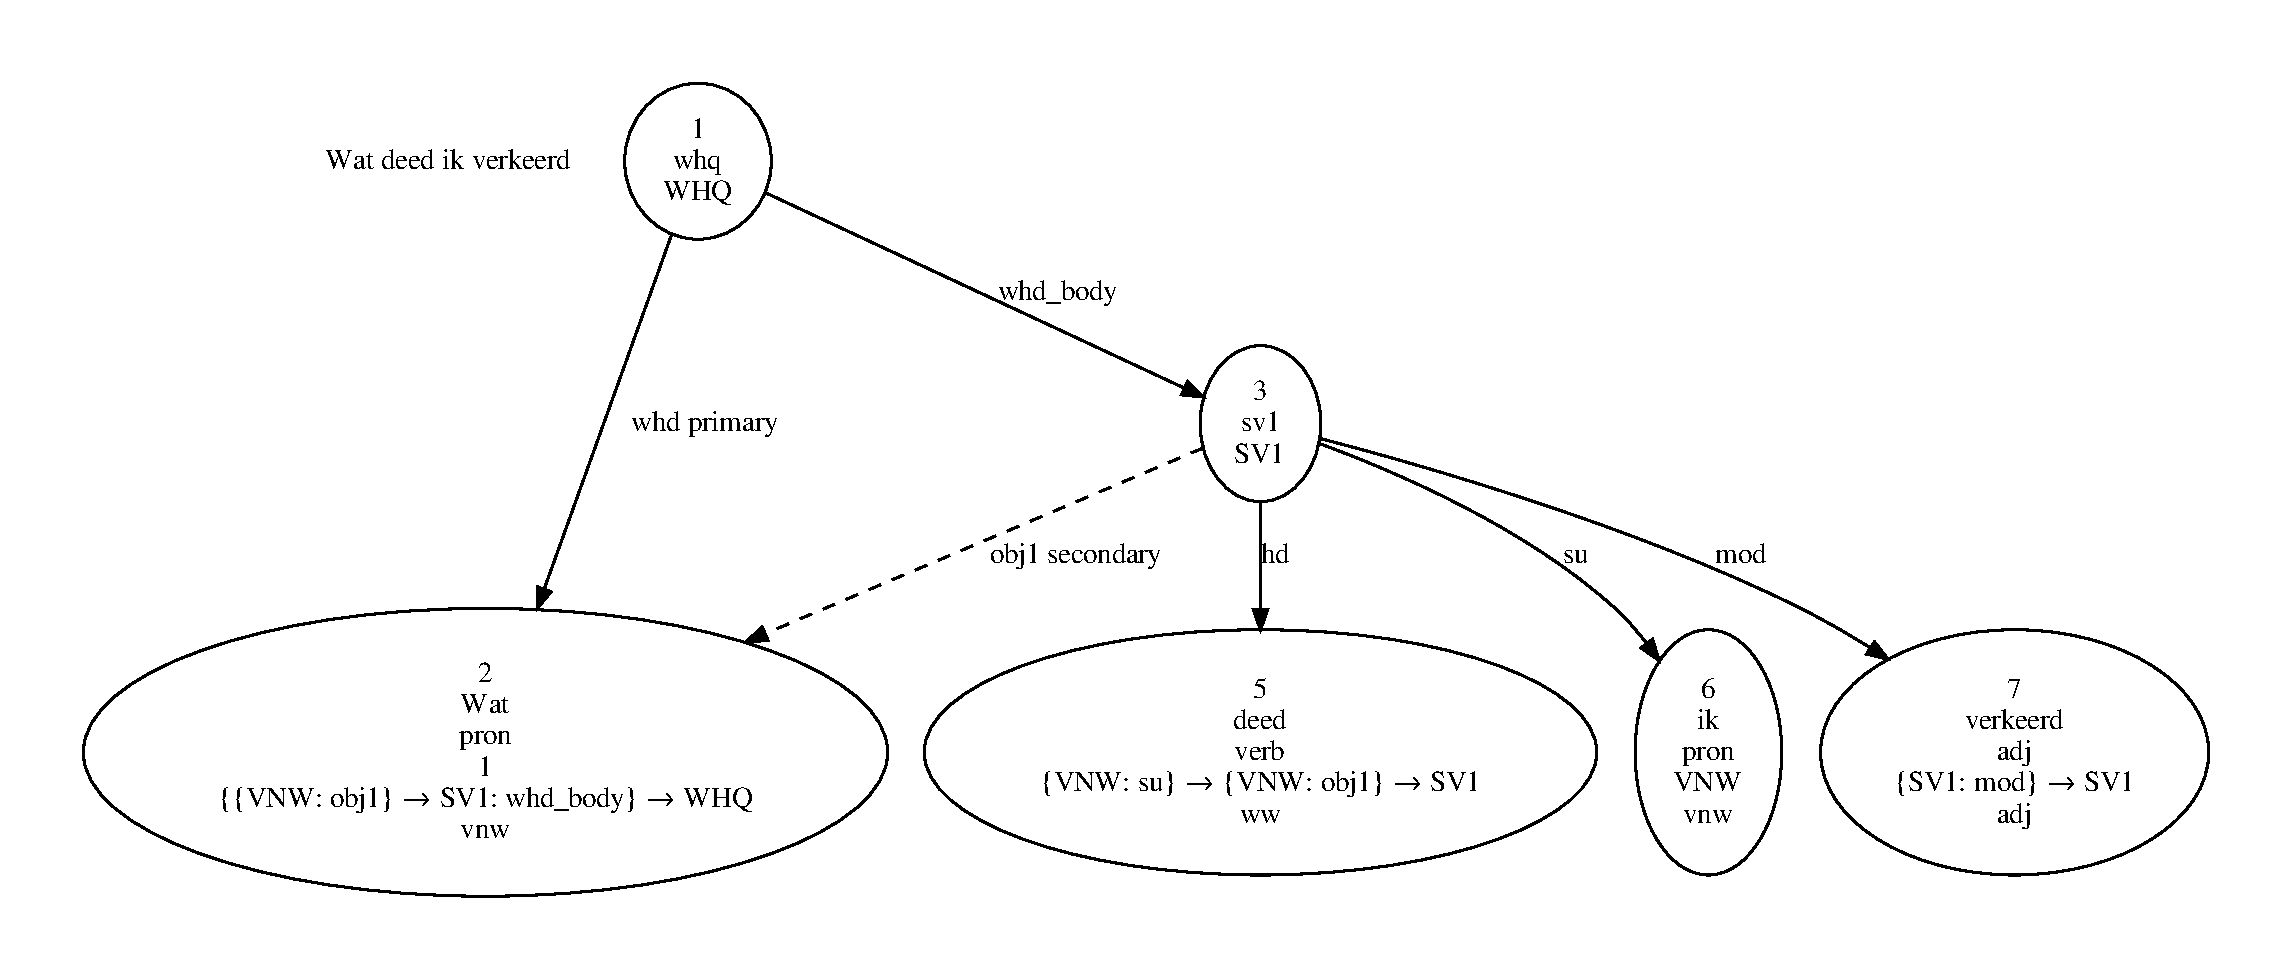
\includegraphics[scale=0.3]{deed2.pdf}
	\end{figure}
\end{frame}
}

\begin{frame}{Extraction: Transformations}
	\begin{itemize}
		\item Majority Voting
		\item Headless Branches
		\item Ellipses
		\item Determiners
	\end{itemize}
\end{frame}

{
\setbeamercolor{background canvas}{bg=gray!00}
\begin{frame}{Extraction: Results (1)}
	\centering
	\vfill
	\textcolor{black}{$\sim$ 5\,700 unique types}
	\begin{figure}
		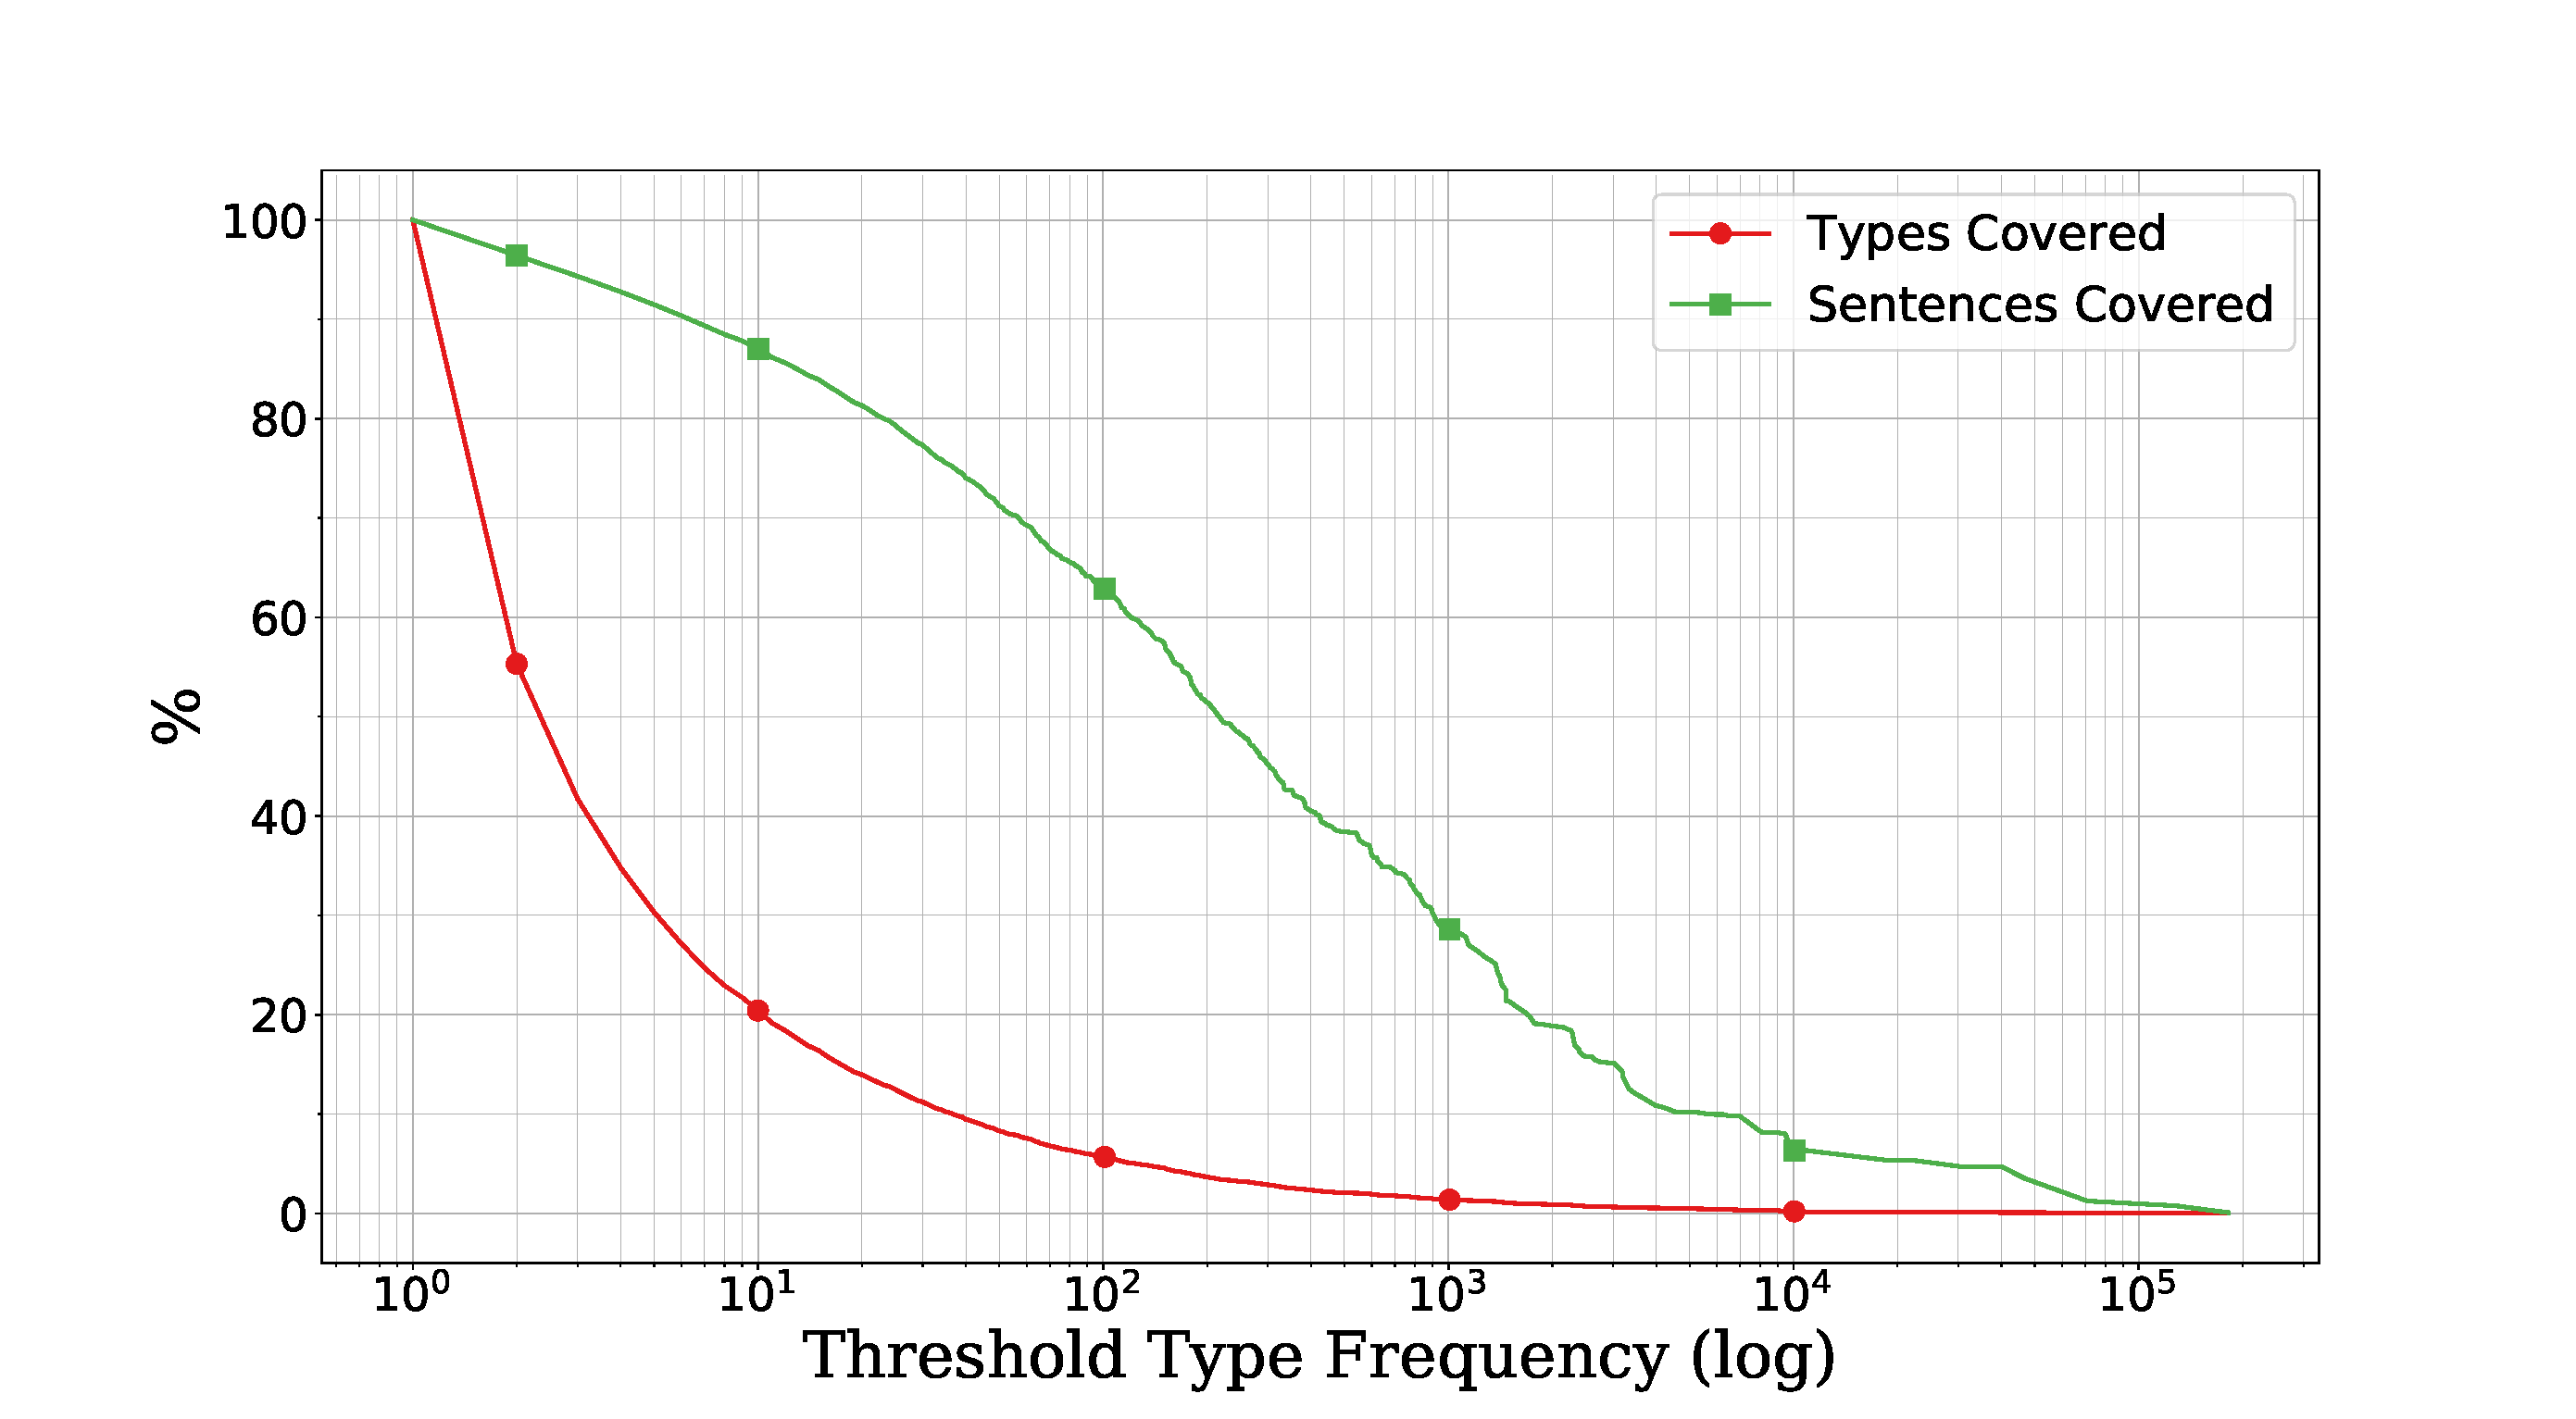
\includegraphics[scale=0.24]{sparsity.pdf}
	\end{figure}
\end{frame}
}

{
\setbeamercolor{background canvas}{bg=gray!00}
\begin{frame}{Extraction: Results (2)}
	\begin{figure}
		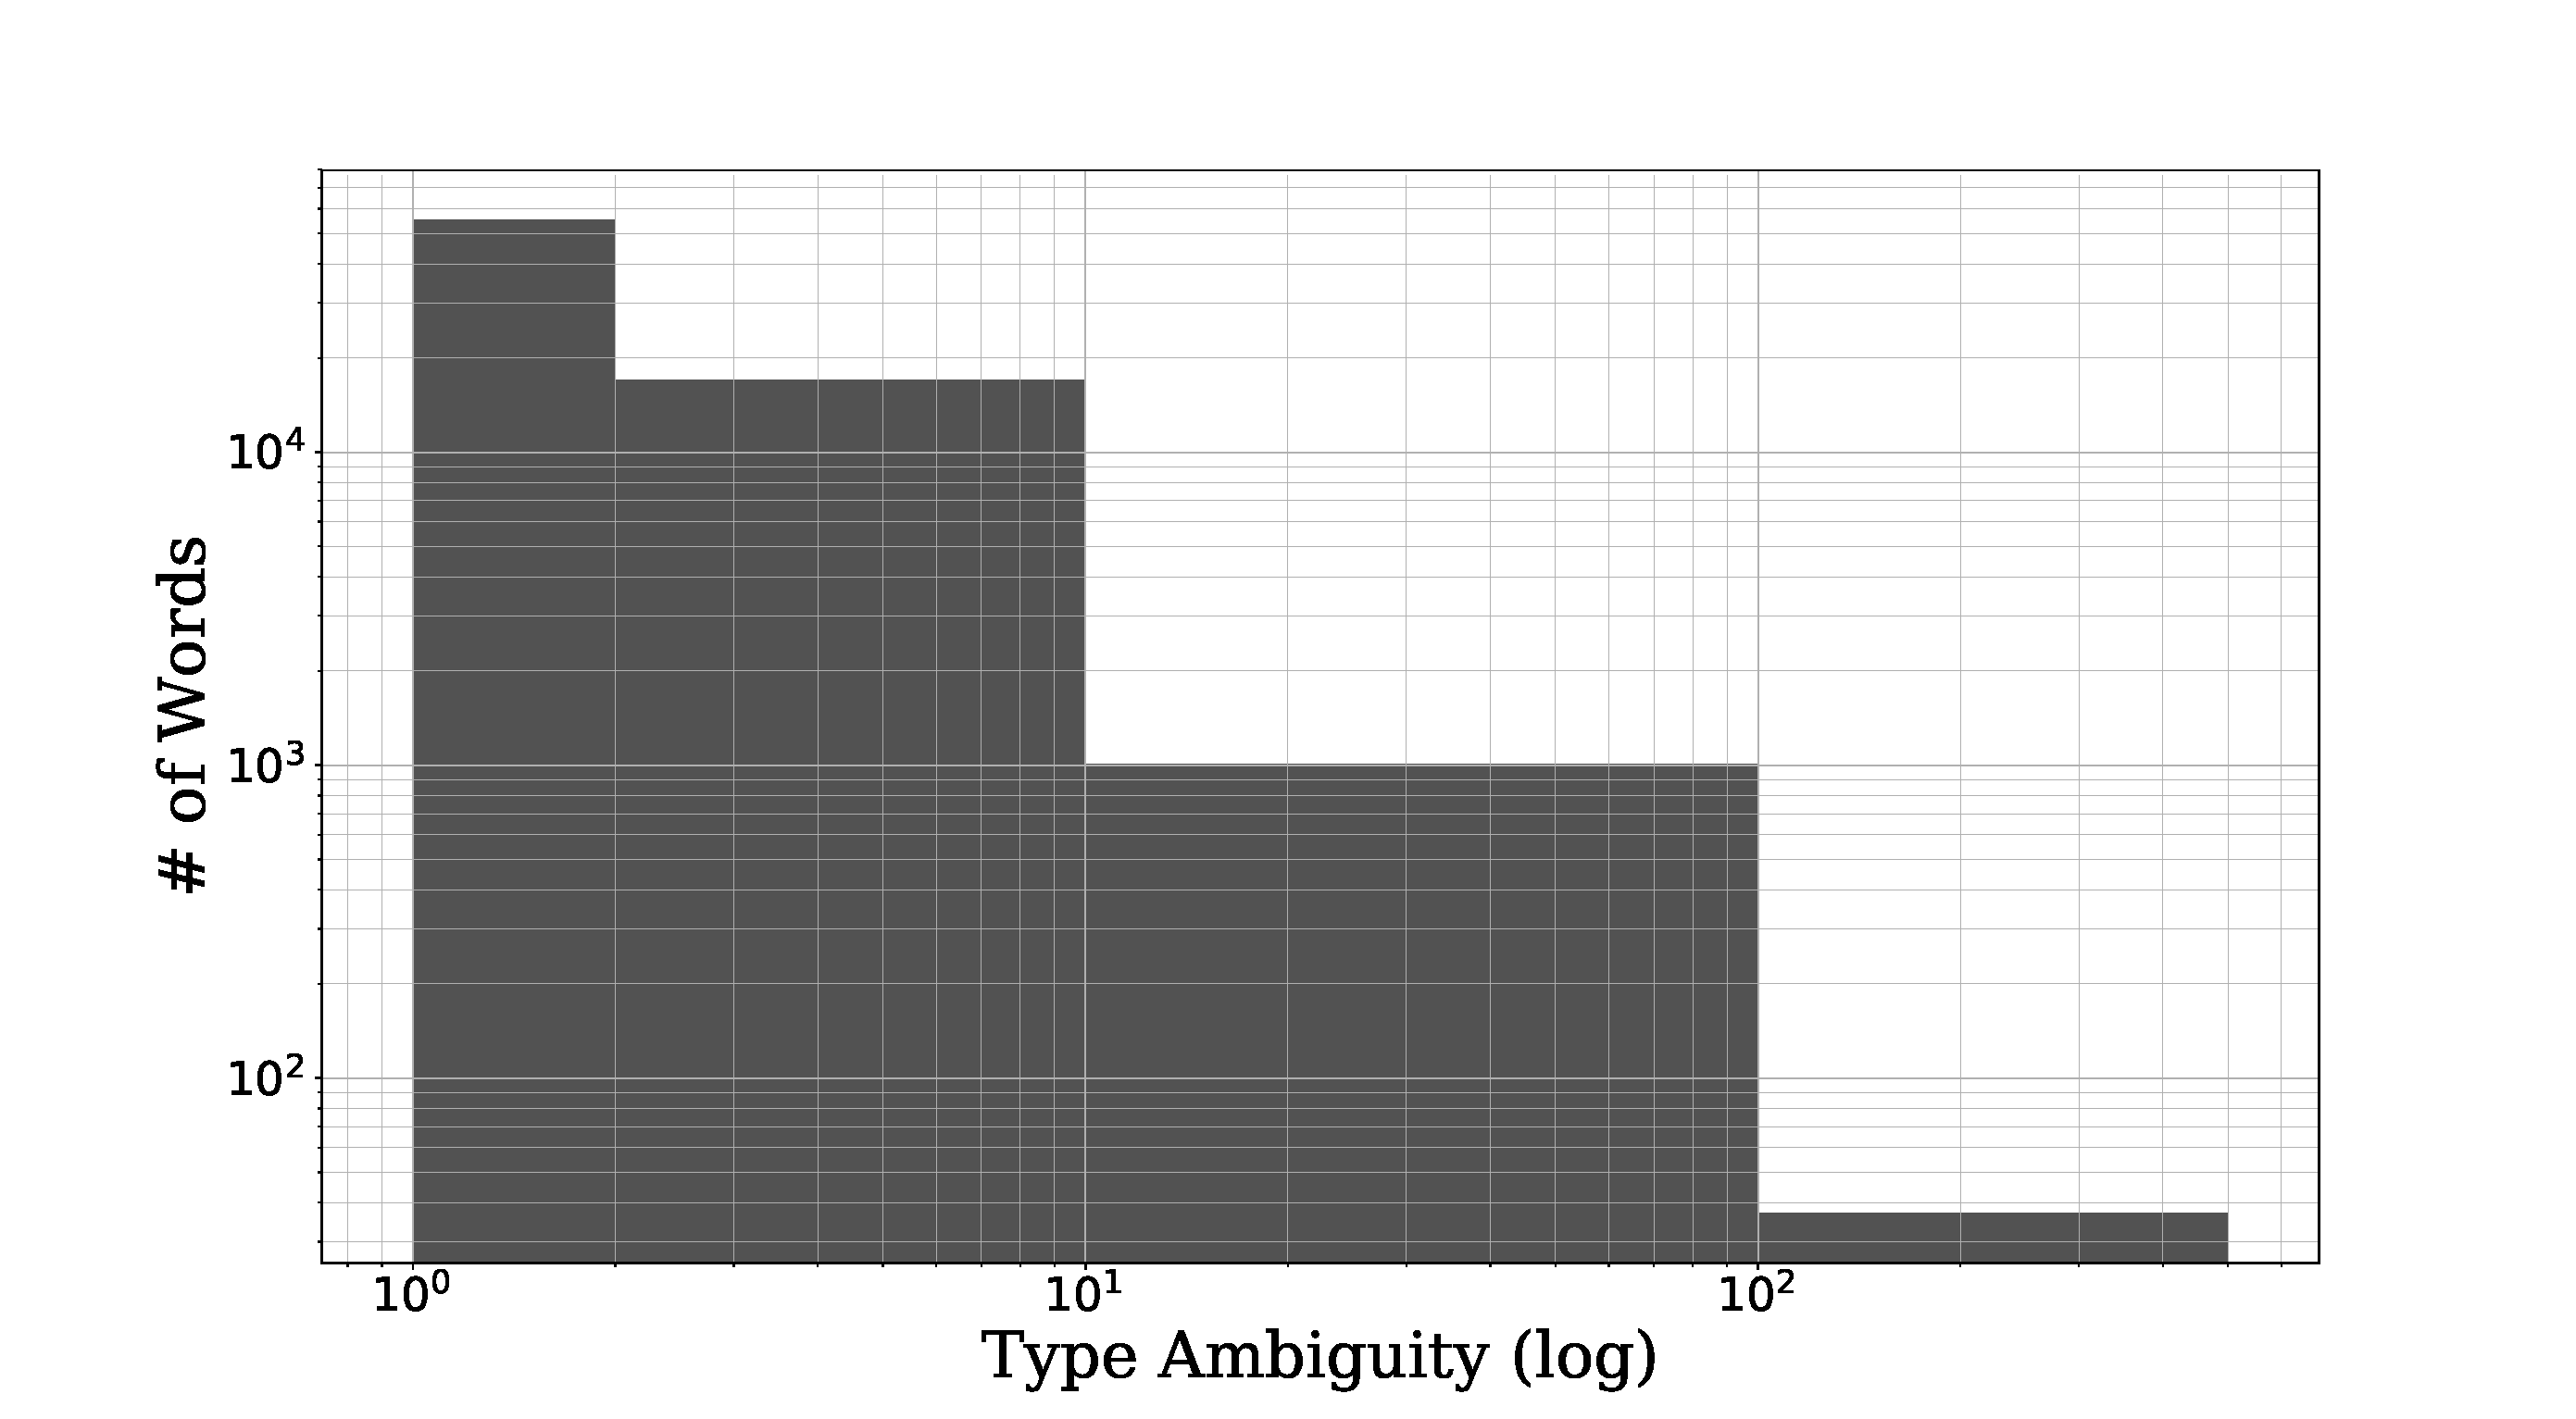
\includegraphics[scale=0.24]{ambiguity.pdf}
	\end{figure}
\end{frame}
}

\section{Supertagging}

\begin{frame}{Supertagging: Standard Approach}
	\alert{Sequence Classification}\\
	\quad Given input data sequence (word vectors) \\
	\quad predict a class for each sequence item (types)
	\vfill
	
	\pause
	\alert{The problem}
	\begin{itemize}
		\item Can't predict unseen items
		\item Difficulty predicting rare items
	\end{itemize}
\end{frame}

\begin{frame}{Supertagging: An Alternative}
	\alert{Type Syntax}\\
	A CFG of two meta-rules
	\begin{align*}
	\{ (S & \implies A) \  \forall \ A \in \mathcal{A} \}\\
	\{(S & \implies d \ S \ S) \ \forall \ d \in \mathcal{D} \}
	\end{align*}
	
	\pause
	CFGs: learnable \\ 
	\pause
	Supertagging: learnable \\
	\pause
	CFG embedded within supertagging $\implies$ \alert{unbounded co-domain}
\end{frame}

\begin{frame}{Supertagging: Unbounded co-domain}

	\alert{Reformulation}\\
	\quad Given input data sequence (word vectors) \\
	\quad generate an output sequence (atomic types \& binary connectives)
	\vfill

	\pause
	\alert{Requirements}
	\begin{itemize}
		\item Global Receptive Field (long-distance dependencies)
		\item Auto-Regressive (output conditional on prior output)	
	\end{itemize}
	
	\alert{Options}
	\begin{itemize}
		\item RNN encoder-decoder \pause \frownie \pause
		\item RNN encoder-separable decoder \pause \frownie \pause
		\item Attentive encoder-decoder \pause \smiley
	\end{itemize}
\end{frame}

\begin{frame}[standout]{Supertagging: Model \& Results}
		\begin{figure}
		\centering
			\scalebox{0.8}{
				\begin{tikzpicture}[every text node part/.style={align=center},
				 every node/.style={transform shape},
				 scale=0.6,
				block/.style={rectangle, inner sep=0pt, minimum width=120pt, minimum height=60pt, rounded corners, ultra thick},
				str/.style={rectangle, inner sep=0pt, minimum width=120pt, minimum height=20pt},
				arrow/.style={->, ultra thick},
				pwise/.style={circle, inner sep=0pt, minimum size=10pt},
				smallblock/.style={circle, inner sep=5pt, minimum size=12pt, rounded corners, thick}]
				
					\node[str] (sentence) at (0, 5) {Input Sentence};		
					\node[str] (symbols) at (7.5, 5) {Output Sequence};
				
				    \definecolor{first}{RGB}{82,82,82}
				    \definecolor{enc}{RGB}{253,192,134}
				    \definecolor{dec}{RGB}{127,201,127}
				    \definecolor{dec2}{RGB}{140,220,140}
				    \definecolor{emb}{RGB}{190,174,212}
				
					\node[block, draw=black, fill=gray!10, draw=gray!130] (elmo) at (0,8) {\textcolor{gray!110}{ELMo}};
					\node[block, draw=black, fill=enc] (te) at (0,12) {\textbf{Encoder}};
					\node[block, draw=black, fill=emb] (se) at (7.5,8) {\textbf{Embedding}};
					\node[block, draw=black, fill=dec2] (td2) at (7.75, 12.25) {};
					\node[block, draw=black, fill=dec] (td) at (7.5,12) {\textbf{Decoder}};
					\node[block, draw=black, fill=emb] (set) at (15,12) {\textbf{Embedding}\\ (transposed)};	
					\node[smallblock, draw=black] (ss) at (15, 8) {$\sigma$};
					\node[smallblock, draw=black] (am) at (12, 8) {$\alpha$};
					\node[str] (out) at (15,5) {Output Probabilities};	
					
				
					\draw (symbols) edge [arrow, gray!130] node[right] {M symbols} (se);
					\draw  (sentence) edge [arrow, gray!130] node[left] {N words} (elmo);
					\draw  (elmo) edge [arrow, gray!130] node[left] {\small Sentence Embedding\\ $\mathbb{R} ^ {N \times 1024}$} (te);
					\draw  (se) edge [arrow] node[right] {\small Symbol Embeddings\\ $\mathbb{R} ^ {M \times 1024}$} (td);
					\draw ($(te.east) + (0, 0.5)$) edge [arrow] node[above] {\small Encoder Keys\\ $\mathbb{R}^ {N \times 1024}$} ($(td.west) + (0, 0.5)$);
					\draw ($(te.east) + (0, -0.5)$) edge [arrow] node[below] {\small Encoder Values\\ $\mathbb{R}^ {N \times 1024}$} ($(td.west) + (0, -0.5)$);\
					\draw ($(td.east) + (0.25, 0)$) edge [arrow] node[above] {\small Decoder Values\\ $\mathbb{R}^ {M \times 1024}$} (set);
					\draw (set) edge [arrow] node[right] {\small Class Weights} (ss);
					\draw (ss) edge [arrow] (out);
					\draw (set.south) [dotted, very thick] .. controls +(-1,0) and +(-0.5, 0.5) .. (am.north);
					\draw (am.south) [dotted, very thick, ->] .. controls +(0,-0.5) and +(2, ) .. (symbols.east);
				\end{tikzpicture}
			}
		\end{figure}
		
		\vfill
		\small
		\hspace{-30pt}
		\begin{tabularx}{0.7\textwidth}{@{}csssss@{}}
			{} & \multicolumn{5}{c}{\centering Frequency}\\
			{} & \small Overall & \small Unseen & \small  Rare & \small Mid & \small High \\
			\cmidrule[0.001em]{2-6}
			Accuracy & \textbf{ 88.05} & \textbf{19.2} & \textbf{45.68} & \textbf{65.62} & 89.93\\
		\end{tabularx}\hfill
		
\end{frame}

\section{Parsing}

\begin{frame}{Parsing: Intro}
	\alert{Goal}\\
	From abstract syntax to surface syntax	
	
	\pause
	\alert{Parse $\equiv$ Proof} \\
	How can we navigate the proof space?
\end{frame}

\begin{frame}{Parsing: General Framework}
	\alert{Parse State}
		\begin{itemize}
			\item[] A logical judgement
			\item[] Word associations for (some) premises
			\item[] A 1-step lookback
		\end{itemize}
		
	\alert{Algorithm}\\
	Given a parse state
	\begin{itemize}
		\item[1] Decide between introduction and elimination
		\item[2] Perform either
		\item[3] Update state(s)
		\item[4] Repeat
	\end{itemize}
\end{frame}

\begin{frame}{Parsing: Elimination}
	Given a sequence of word \& type pairs \\ 
	\quad Split into two disjoint sequences.. \\
	\pause
	\quad ..by assigning each item one of two labels
\end{frame}

\begin{frame}{Parsing: Model}
	\begin{figure}
	\end{figure}
\end{frame}

\end{document}